\begin{figure}[htp]
\begin{center}
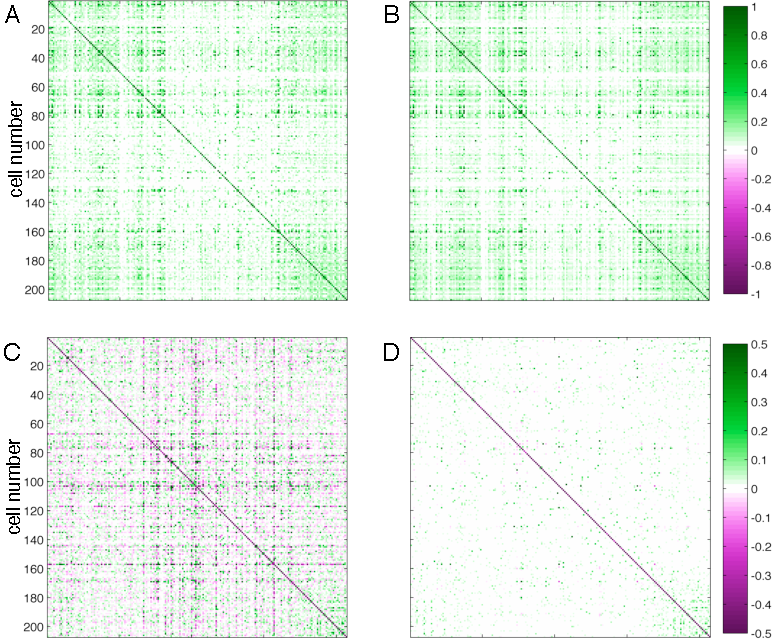
\includegraphics[width=0.5\textwidth]{figures/Figure0.pdf}
\end{center}
\caption{
{\bf An illustration of regularized estimaton of the covariance matrix.}  \TODO{generate a smaller and simple example}
{\bf A:} The sample covariance matrix of population calcium signals of 204 cells.
{\bf B:} The sample precison matrix (inverse of the sample covariance matrix in {\bf B}.
{\bf C:} A estimate of the covariance matrix produced by bounding the $L_1$ norm of the precision matrix. 
{\bf D:} The precision matrix of the estimate in {\bf C}.
}
\label{fig:00}
\end{figure}
